\chapter{Appendix}
\label{sec:Appendix}
% Hier greift man einige wenige, interessante Gesichtspunkte der
% Implementierung heraus. Das Kapitel darf nicht mit Dokumentation oder
% gar Programmkommentaren verwechselt werden. Es kann vorkommen, daß
% sehr viele Gesichtspunkte aufgegriffen werden müssen, ist aber nicht
% sehr häufig. Zweck dieses Kapitels ist einerseits, glaubhaft zu
% machen, daß man es bei der Arbeit nicht mit einem "Papiertiger"
% sondern einem real existierenden System zu tun hat. Es ist sicherlich
% auch ein sehr wichtiger Text für jemanden, der die Arbeit später
% fortsetzt. Der dritte Gesichtspunkt dabei ist, einem Leser einen etwas
% tieferen Einblick in die Technik zu geben, mit der man sich hier
% beschäftigt. Schöne Bespiele sind "War Stories", also Dinge mit denen
% man besonders zu kämpfen hatte, oder eine konkrete, beispielhafte
% Verfeinerung einer der in Kapitel 3 vorgestellten Ideen. Auch hier
% gilt, mehr als 20 Seiten liest keiner, aber das ist hierbei nicht so
% schlimm, weil man die Lektüre ja einfach abbrechen kann, ohne den
% Faden zu verlieren. Vollständige Quellprogramme haben in einer Arbeit
% nichts zu suchen, auch nicht im Anhang, sondern gehören auf Rechner,
% auf denen man sie sich ansehen kann.

\begin{figure}[tbp]
  \centering
  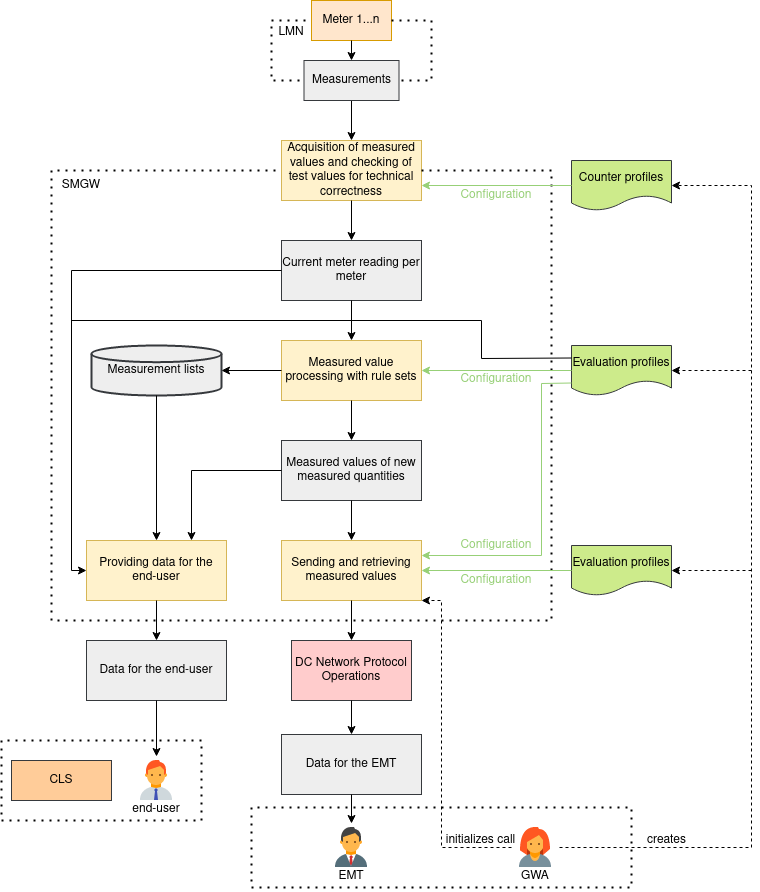
\includegraphics[width=1\textwidth]{images/Messverarbeitung_mit_DC_Eng.png}
  \caption[Measured Value Processing in a SMGW]{An overview of the measured value processing within the SMGW with configuration profiles from the GWA and DC Network Protocol Extension.}
  \label{fig:value_processing_with_dc}
\end{figure}

\afterpage{%
\begin{figure}[!p]
\centering
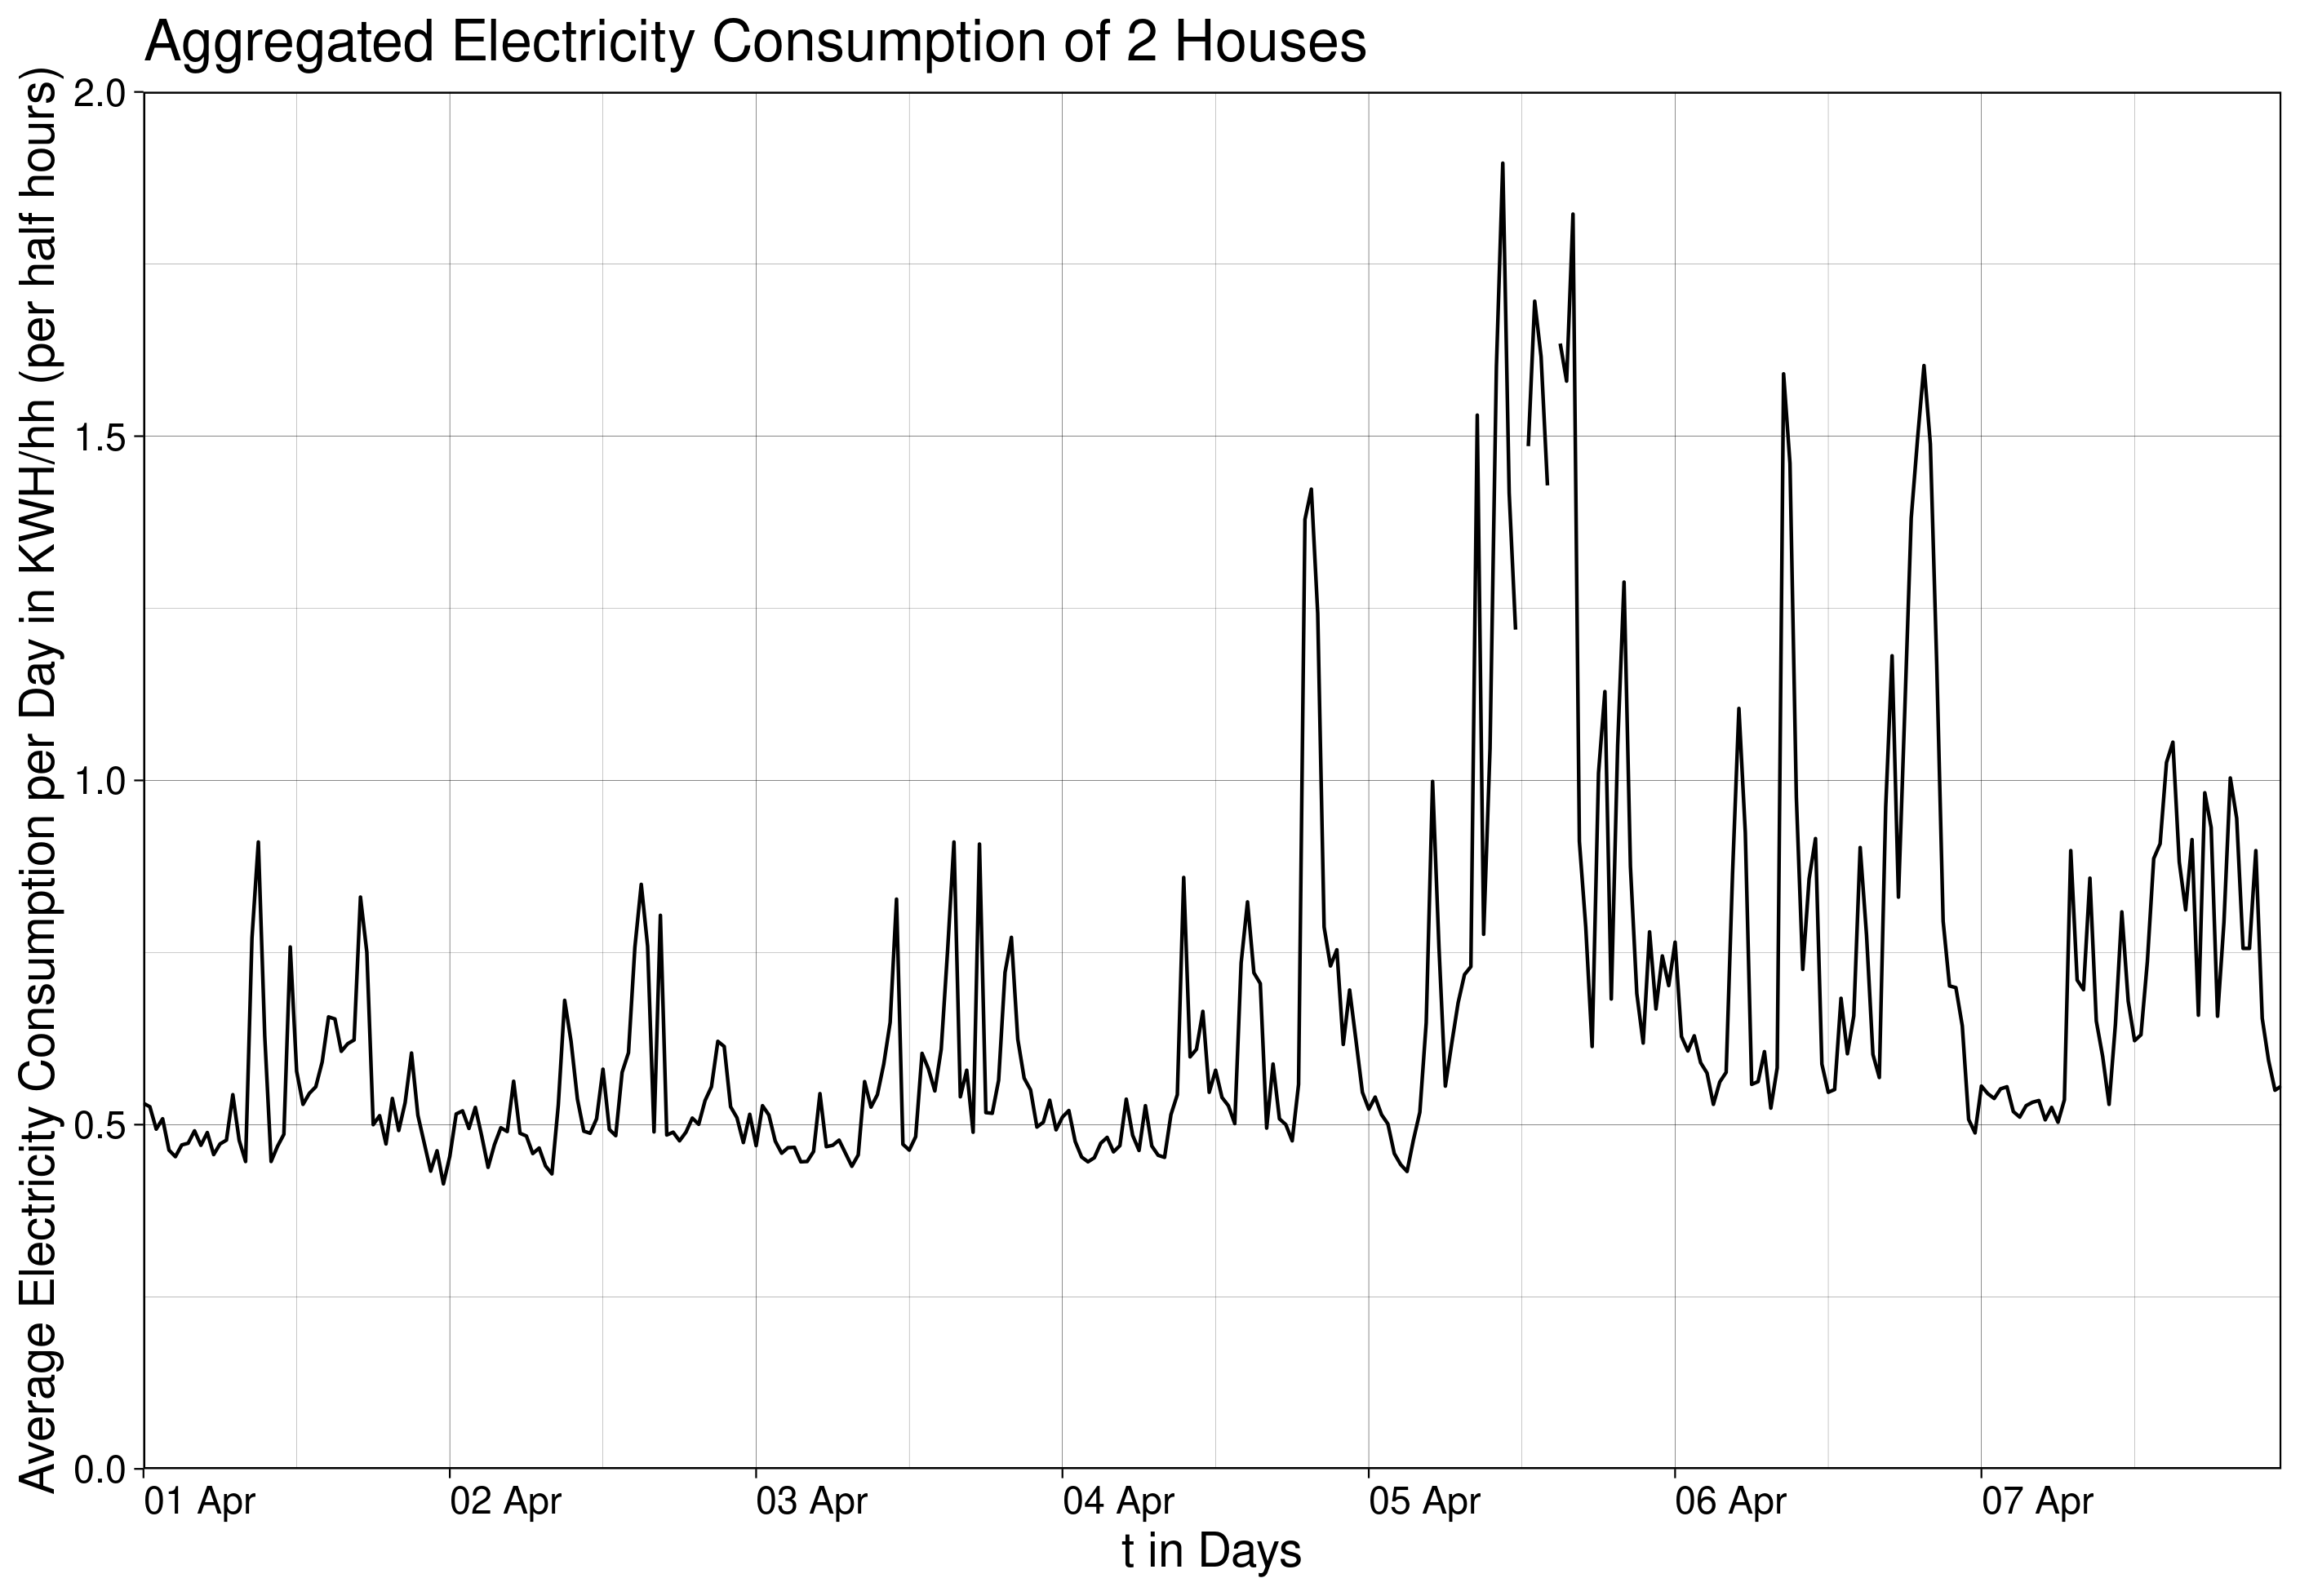
\includegraphics[width=0.85\textwidth]{images/Aggregated Electricity Consumption of 2 Houses6.png}
\caption[Aggregated Electricity Consumption of 2 Houses of the 2nd Experiment of the 2nd Experiment]{}
\label{img:2_Houses_weekly}
\end{figure}
\begin{figure}[!p]
\centering
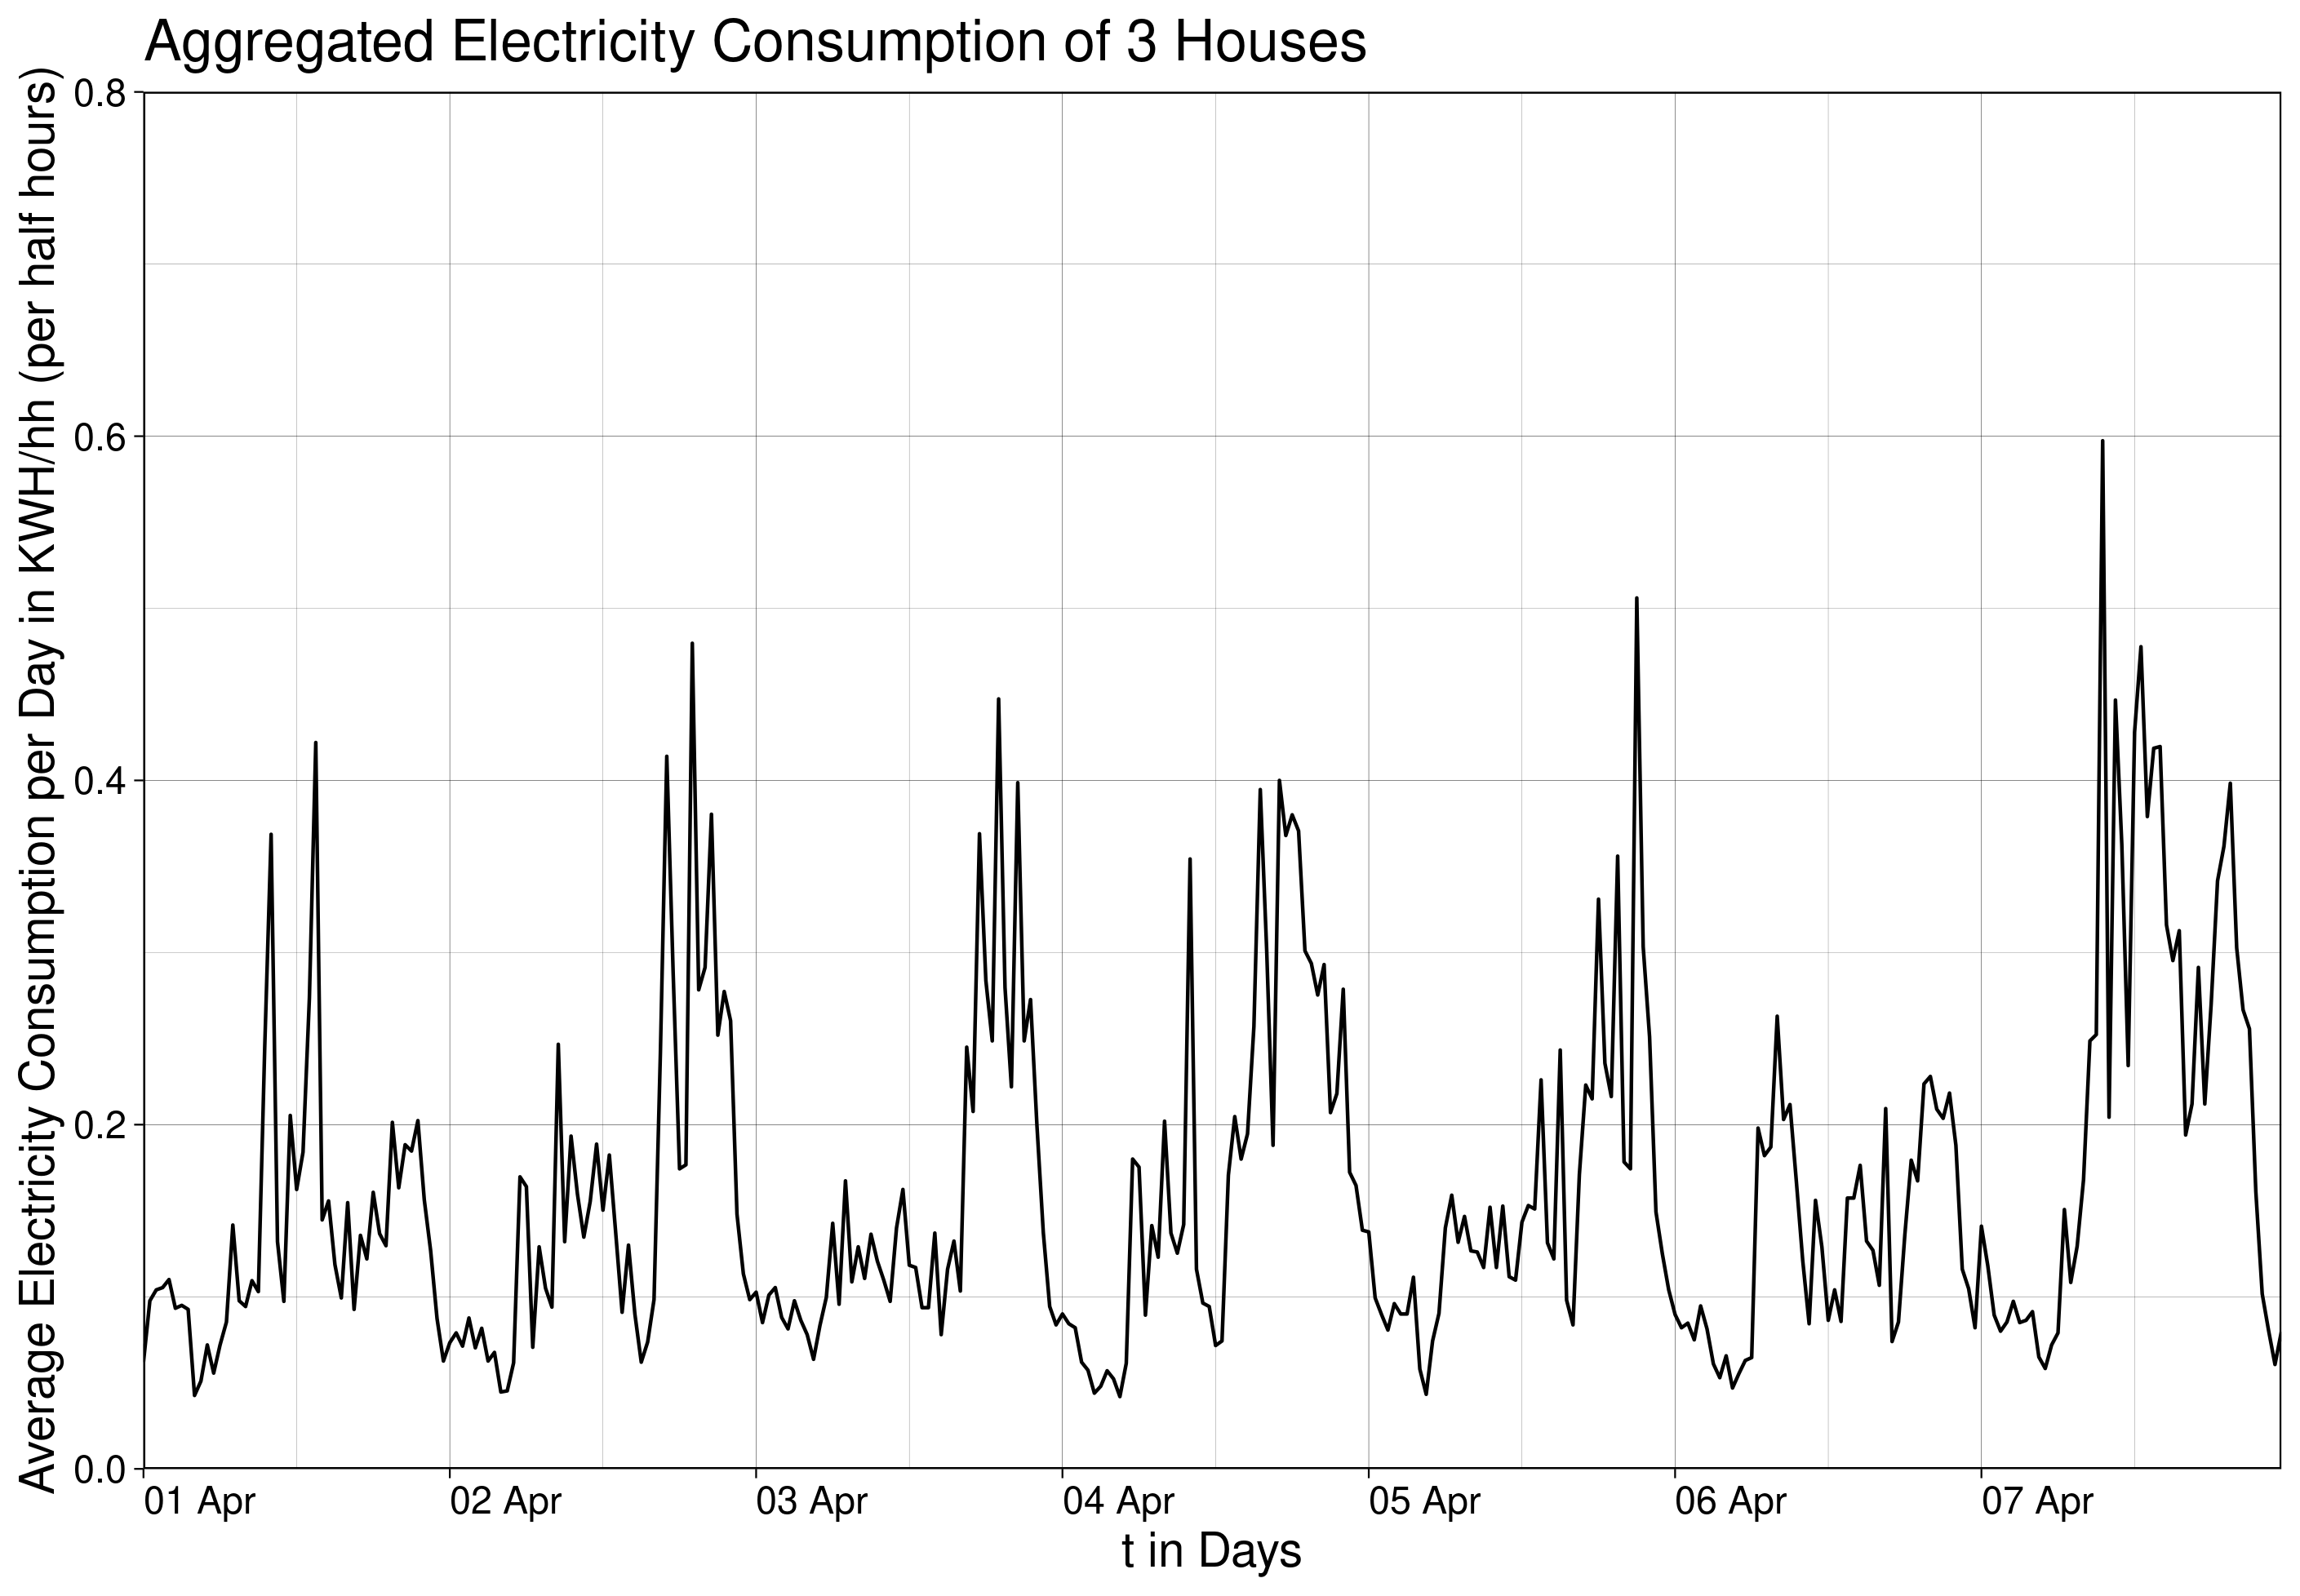
\includegraphics[width=0.85\textwidth]{images/Aggregated Electricity Consumption of 3 Houses5.png}
\caption[Aggregated Electricity Consumption of 3 Houses of the 2nd Experiment]{}
\label{img:3_Houses_weekly}
\end{figure}
\clearpage
}
\afterpage{%
\begin{figure}[!p]
\centering
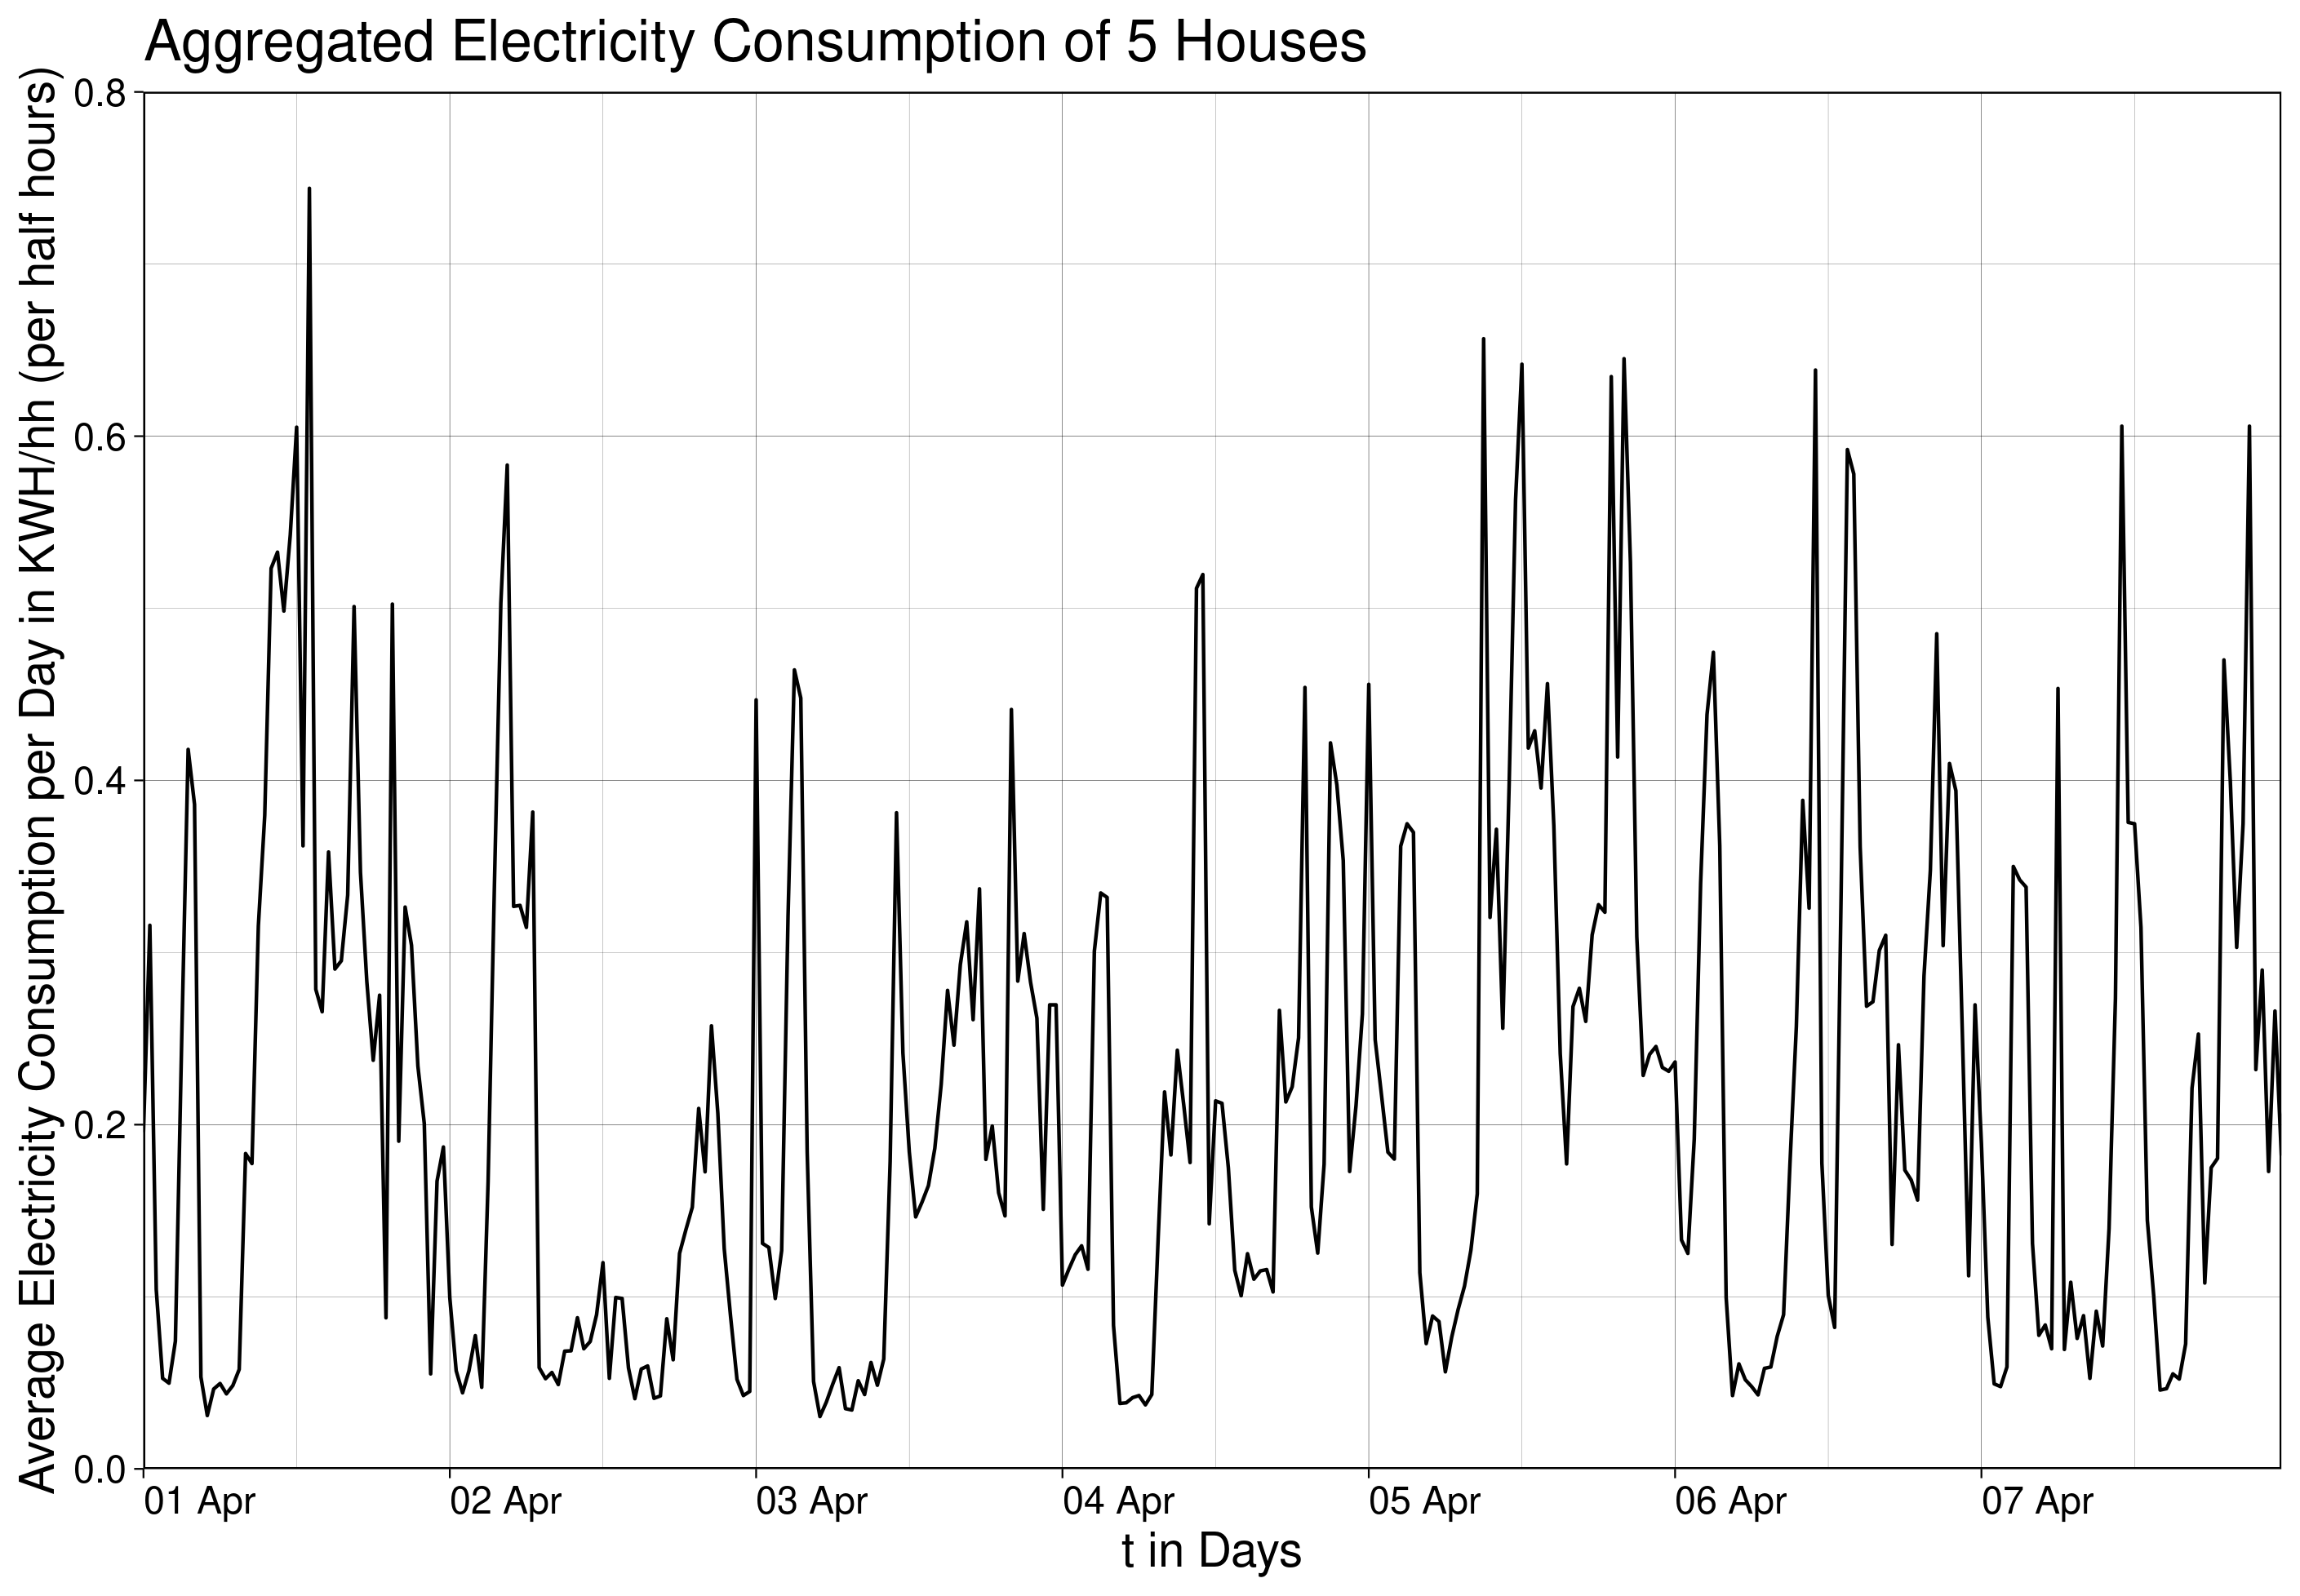
\includegraphics[width=0.85\textwidth]{images/Aggregated Electricity Consumption of 5 Houses5.png}
\caption[Aggregated Electricity Consumption of 5 Houses of the 2nd Experiment]{}
\label{img:5_Houses_weekly}
\end{figure}
\begin{figure}[!p]
\centering
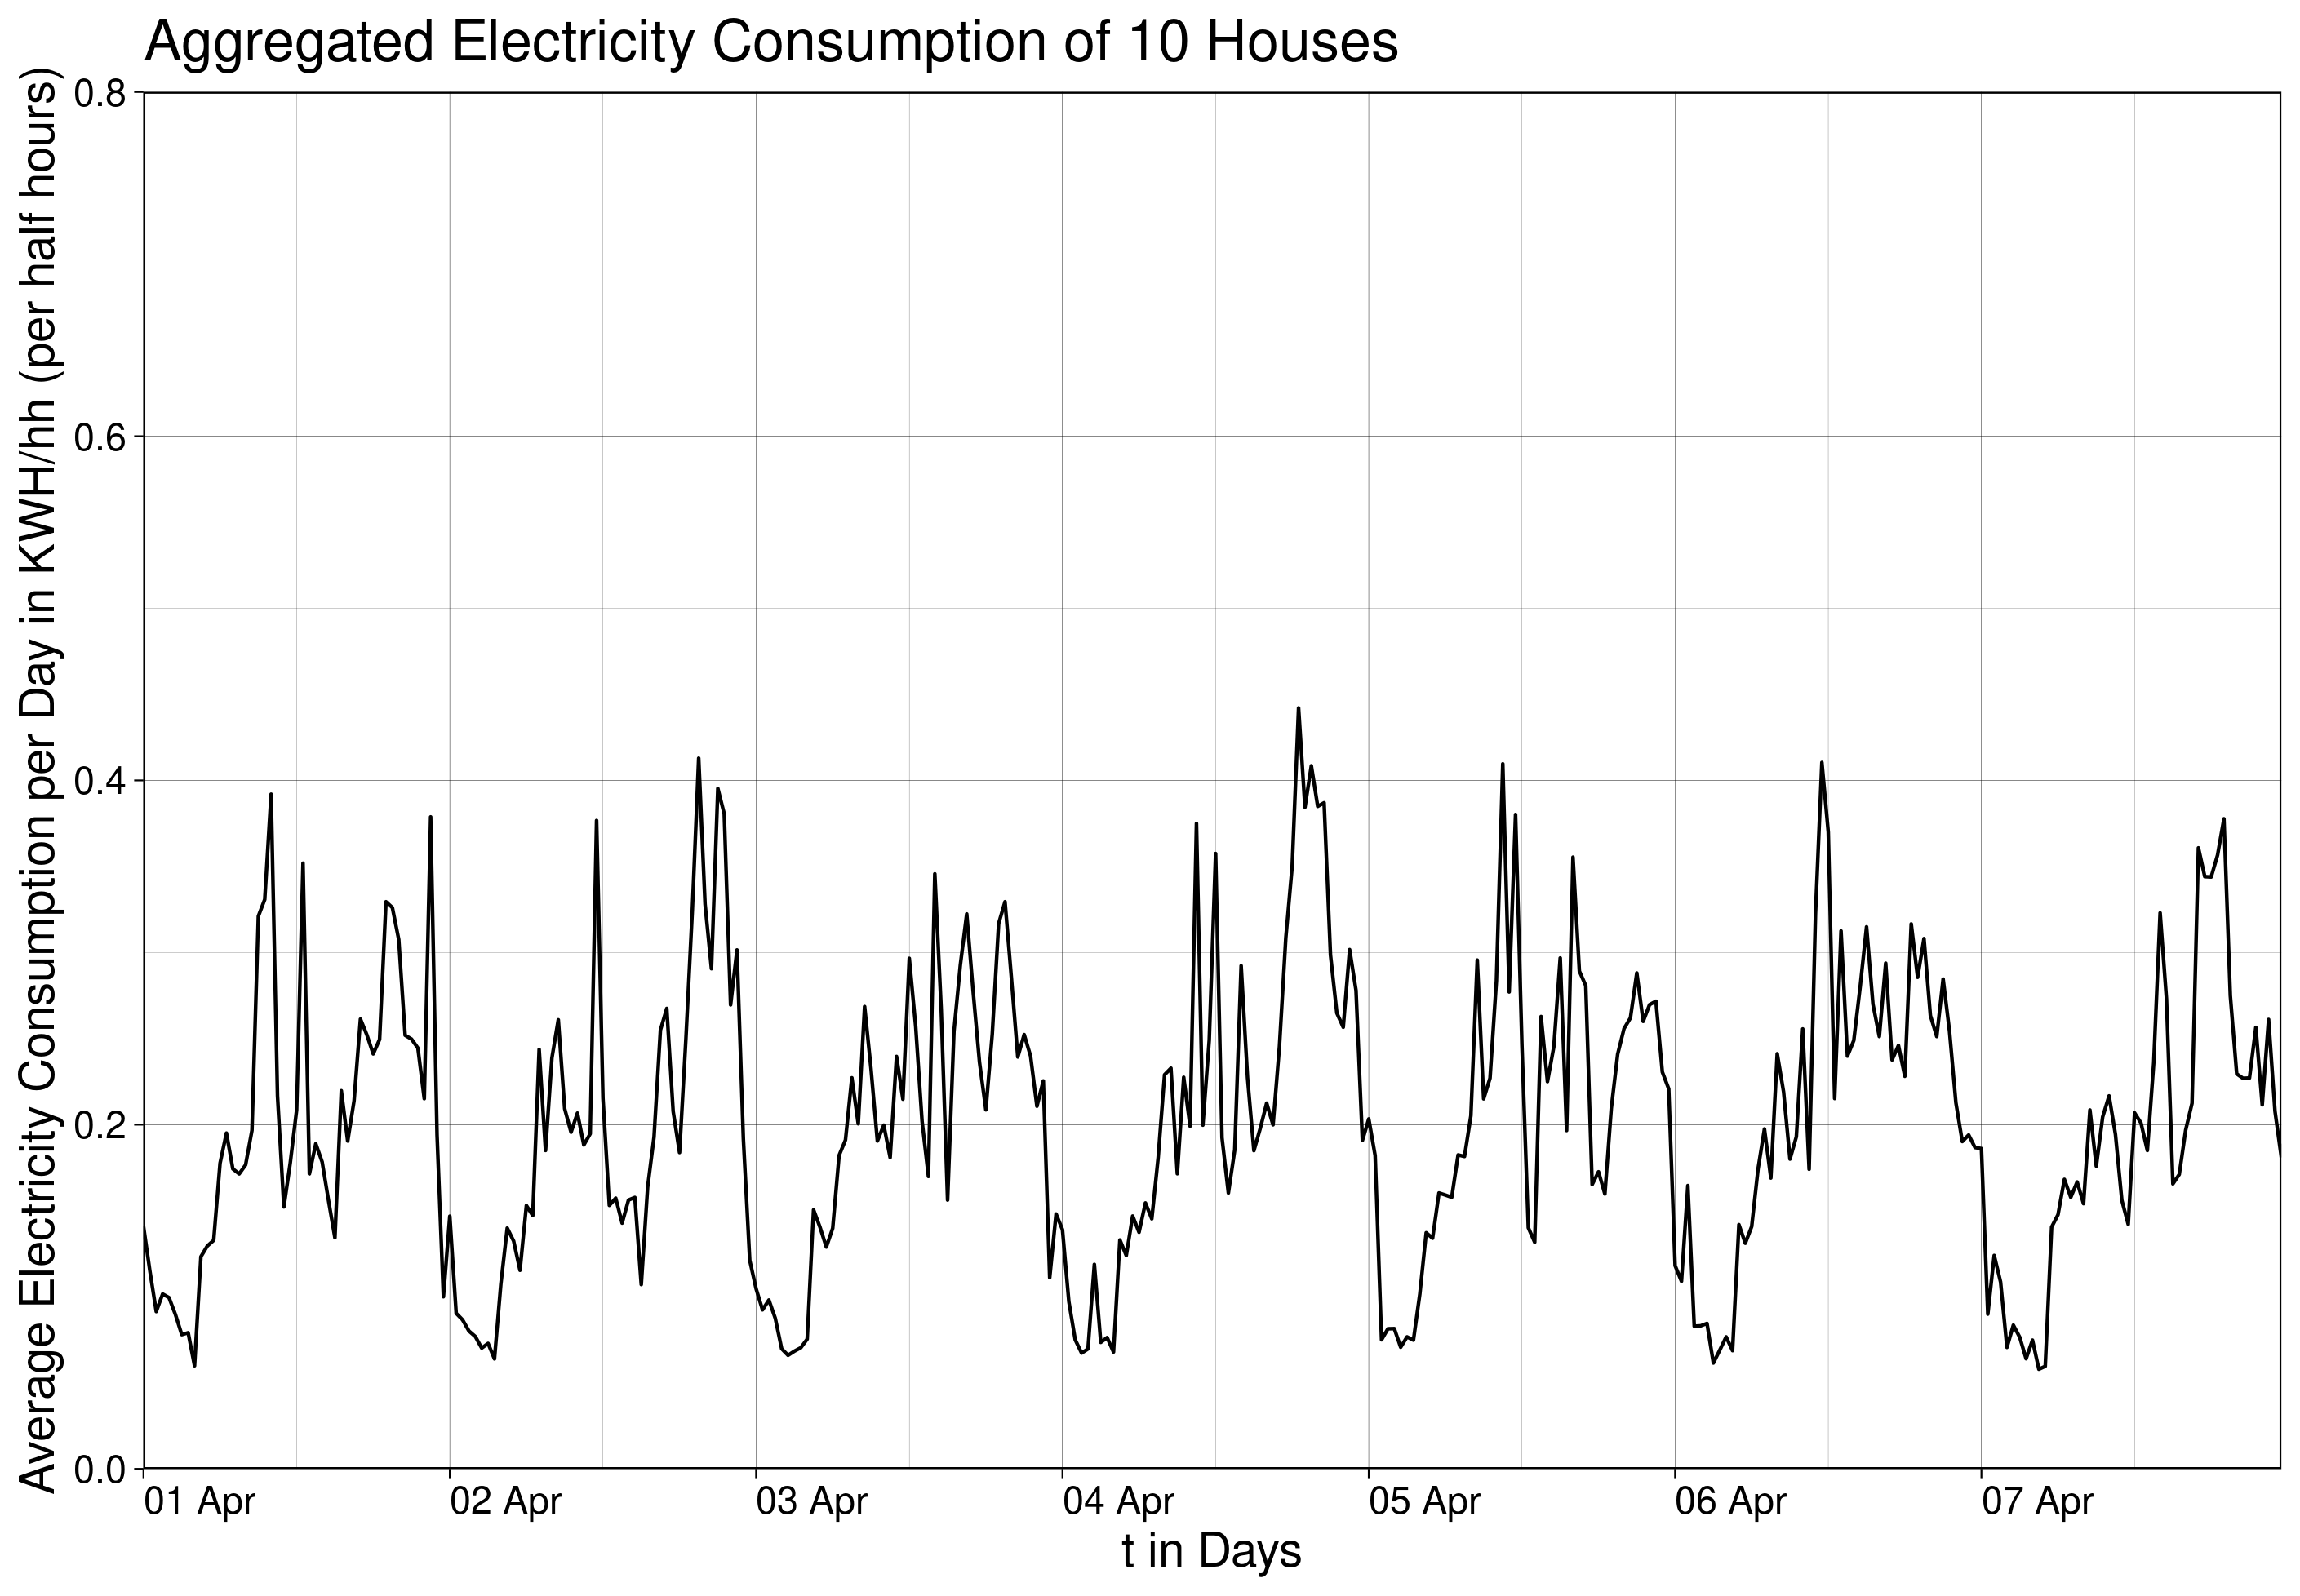
\includegraphics[width=0.85\textwidth]{images/Aggregated Electricity Consumption of 10 Houses5.png}
\caption[Aggregated Electricity Consumption of 10 Houses of the 2nd Experiment]{}
\label{img:10_Houses_weekly}
\end{figure}
\clearpage
}
\afterpage{%
\begin{figure}[!p]
\centering
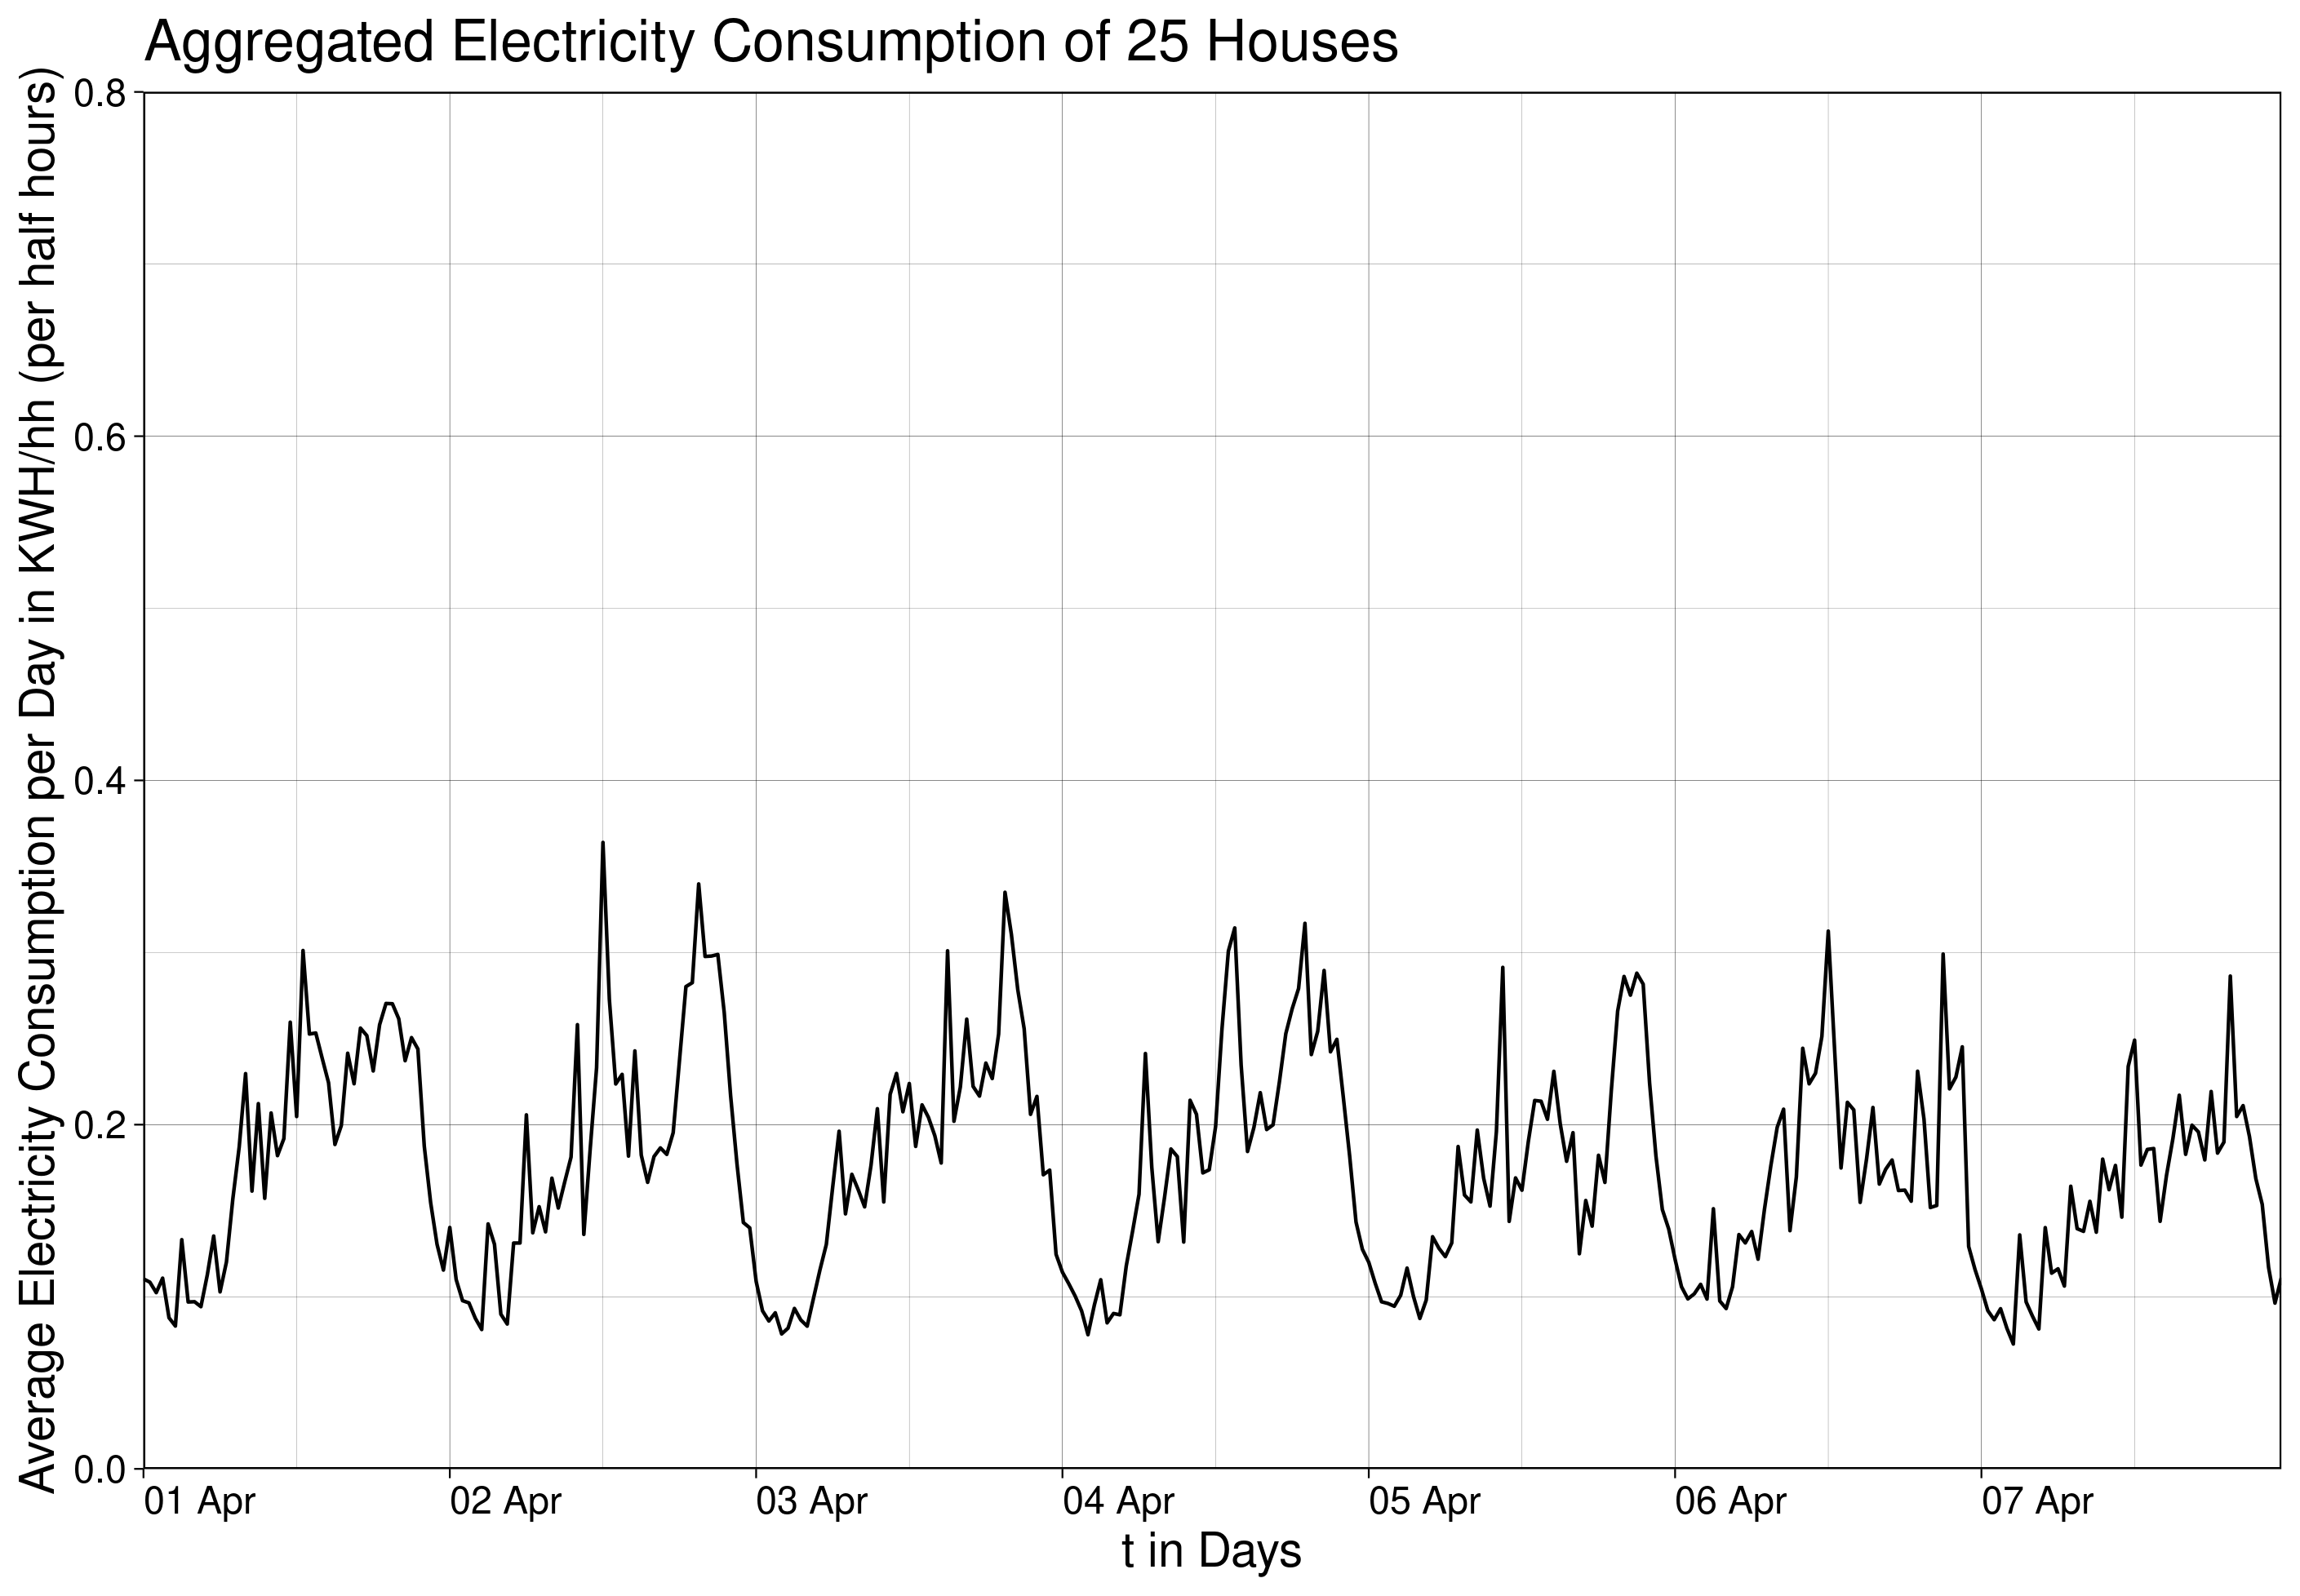
\includegraphics[width=0.85\textwidth]{images/Aggregated Electricity Consumption of 25 Houses5.png}
\caption[Aggregated Electricity Consumption of 25 Houses of the 2nd Experiment]{}
\label{img:25_Houses_weekly}
\end{figure}
\begin{figure}[!p]
\centering
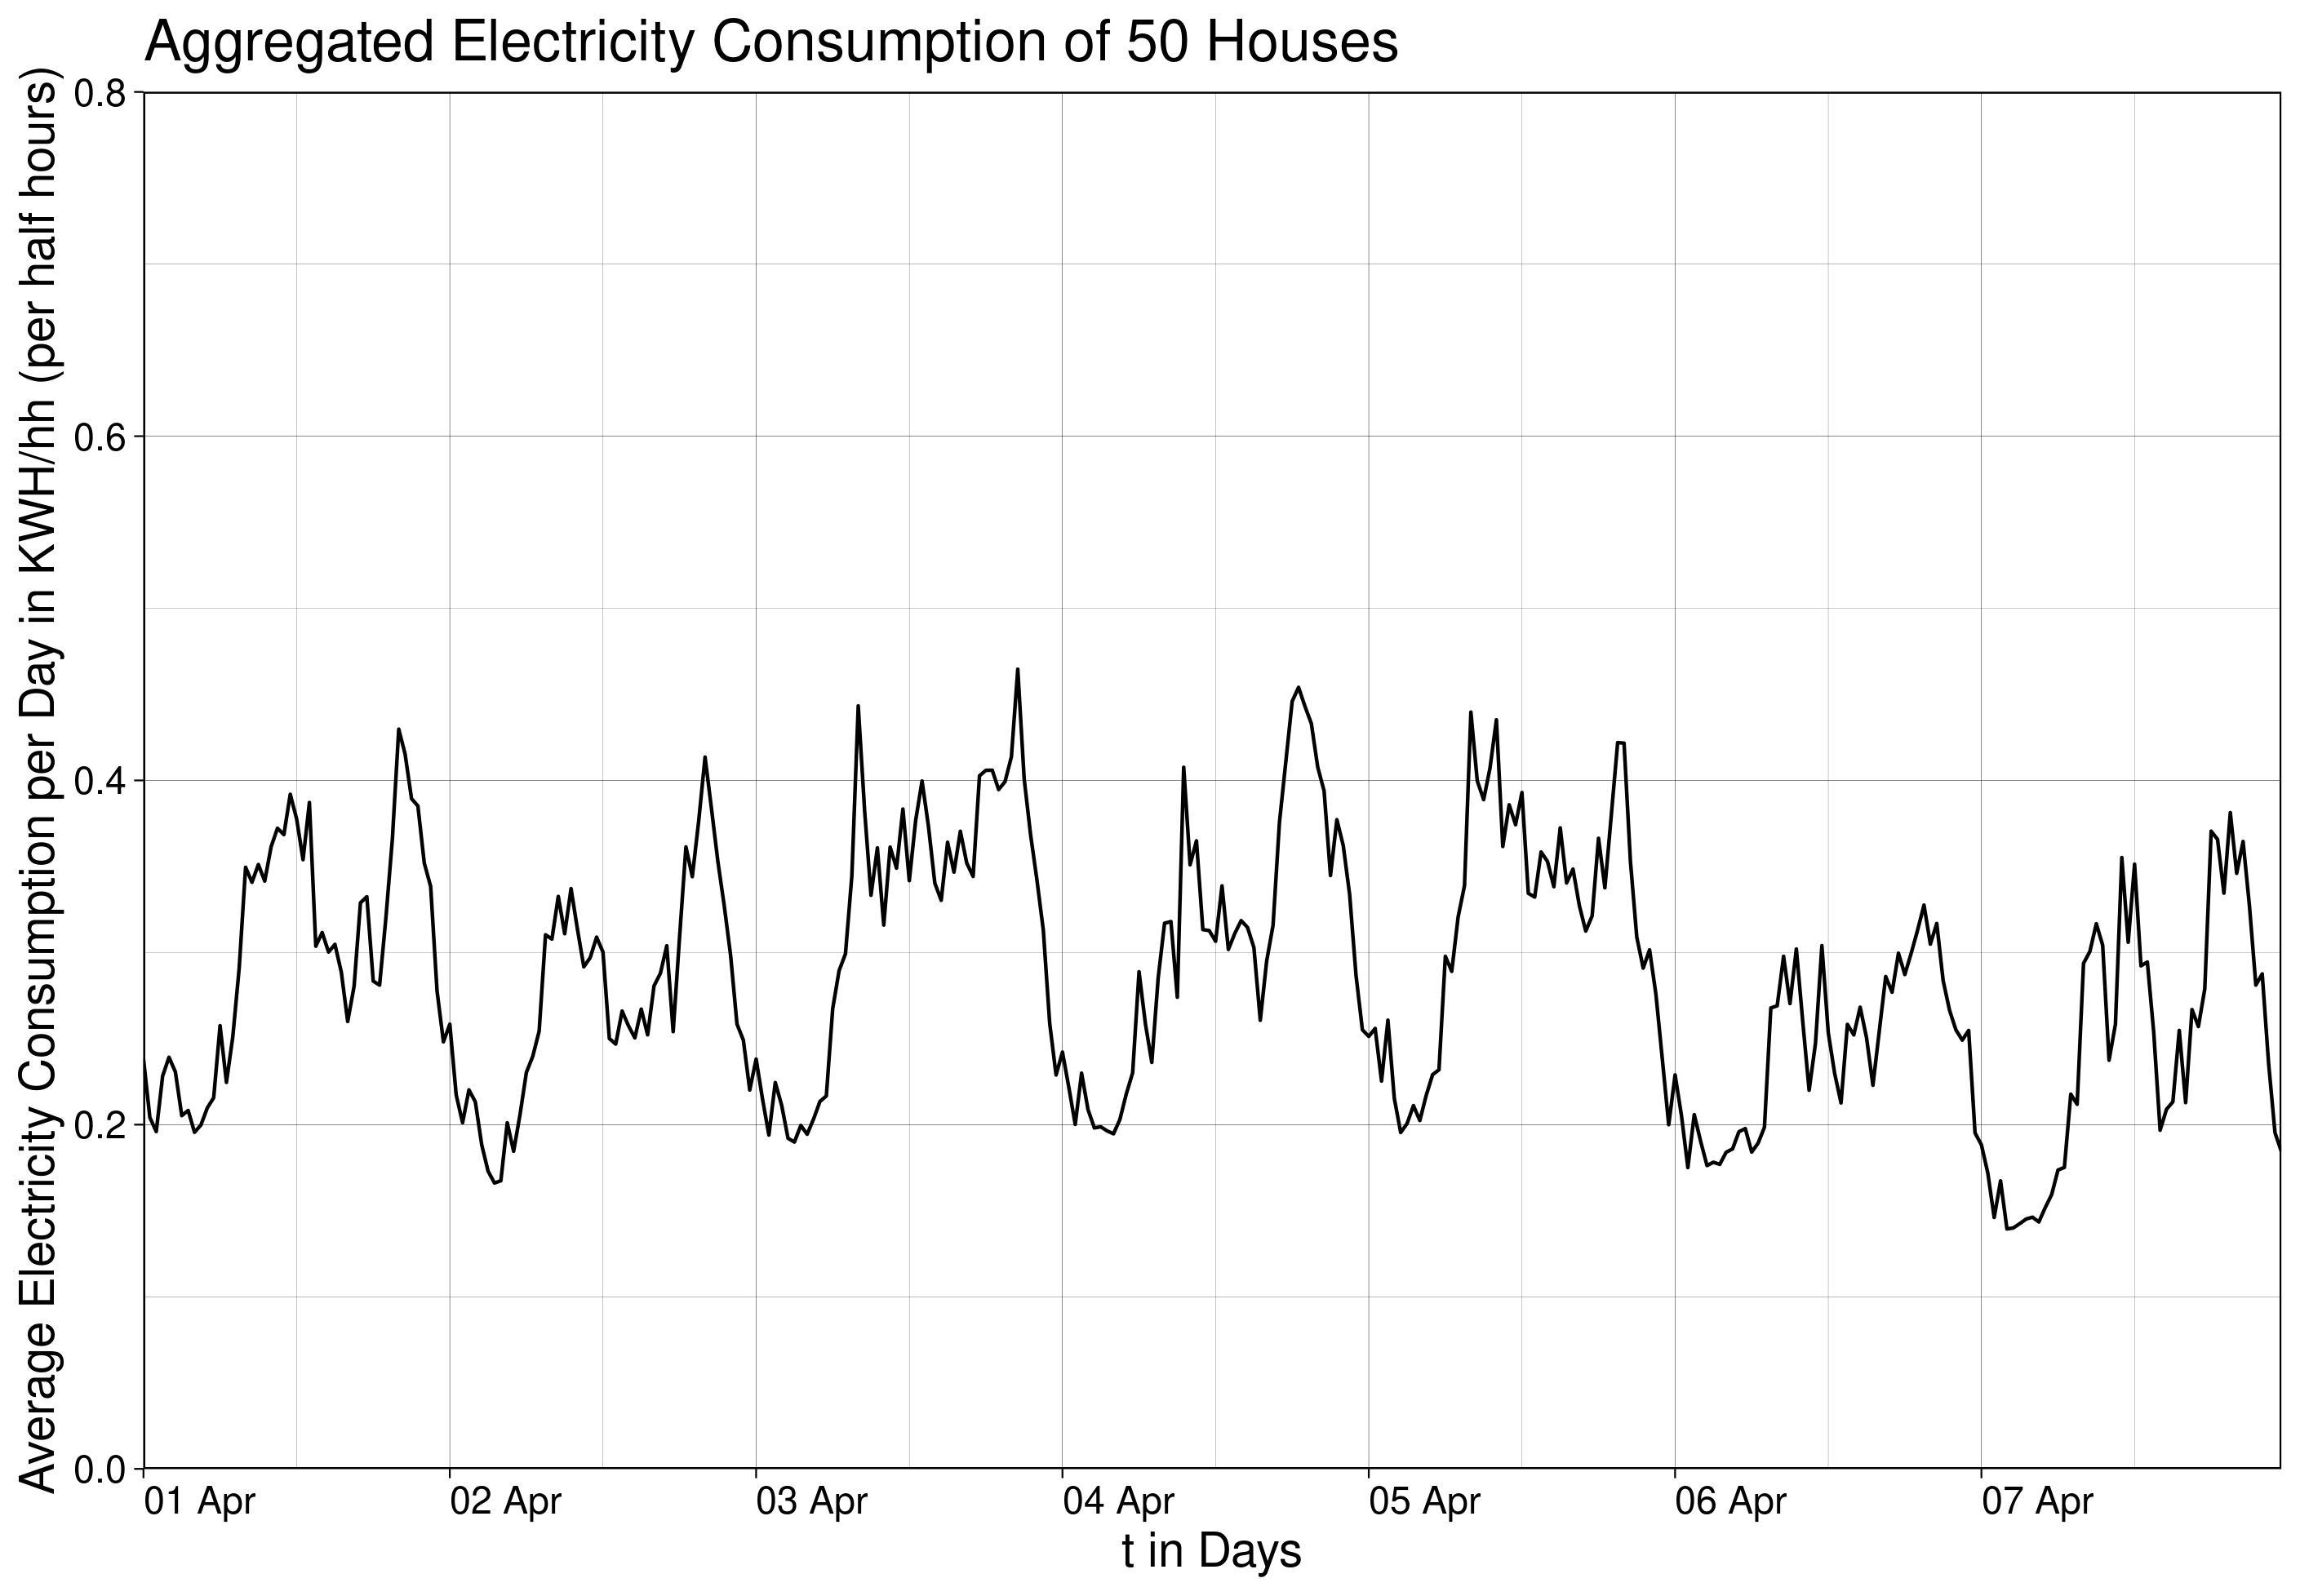
\includegraphics[width=0.85\textwidth]{images/Aggregated Electricity Consumption of 50 Houses5.png}
\caption[Aggregated Electricity Consumption of 50 Houses of the 2nd Experiment]{}
\label{img:50_Houses_weekly}
\end{figure}
\clearpage
}
\afterpage{%
\begin{figure}[!p]
\centering
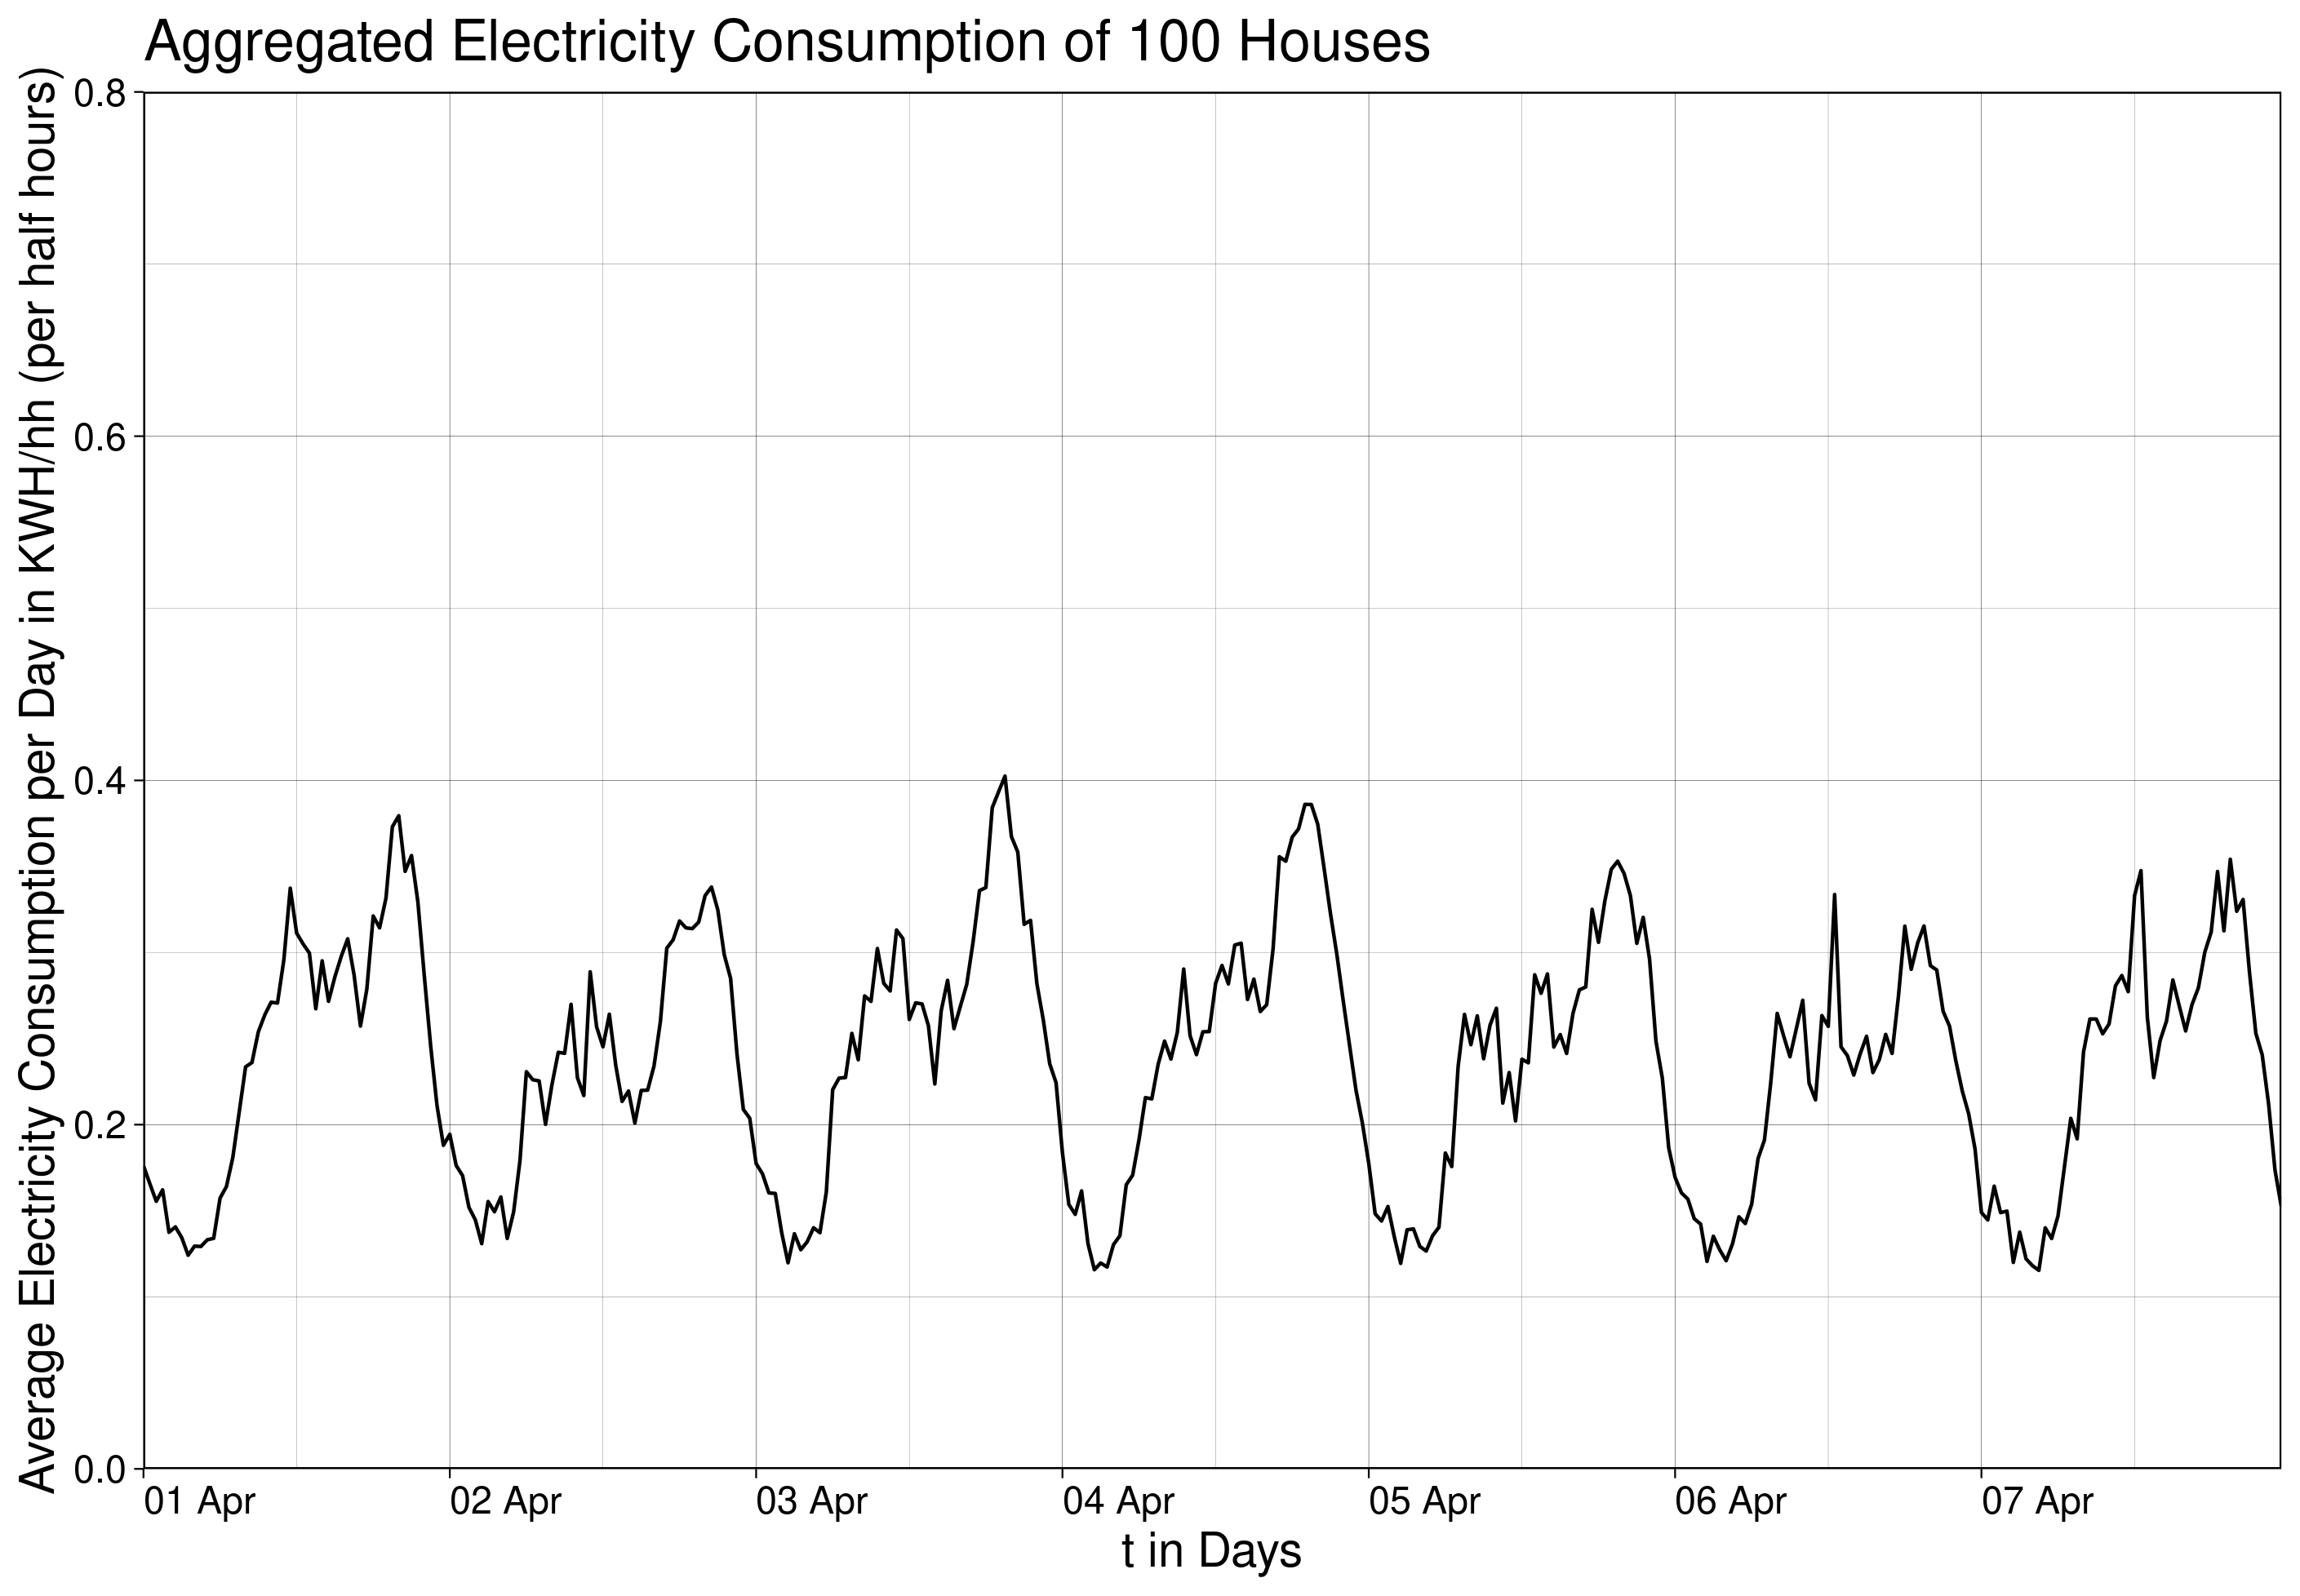
\includegraphics[width=0.85\textwidth]{images/Aggregated Electricity Consumption of 100 Houses5.png}
\caption[Aggregated Electricity Consumption of 100 Houses of the 2nd Experiment]{}
\label{img:100_Houses_weekly}
\end{figure}
\begin{figure}[!p]
\centering
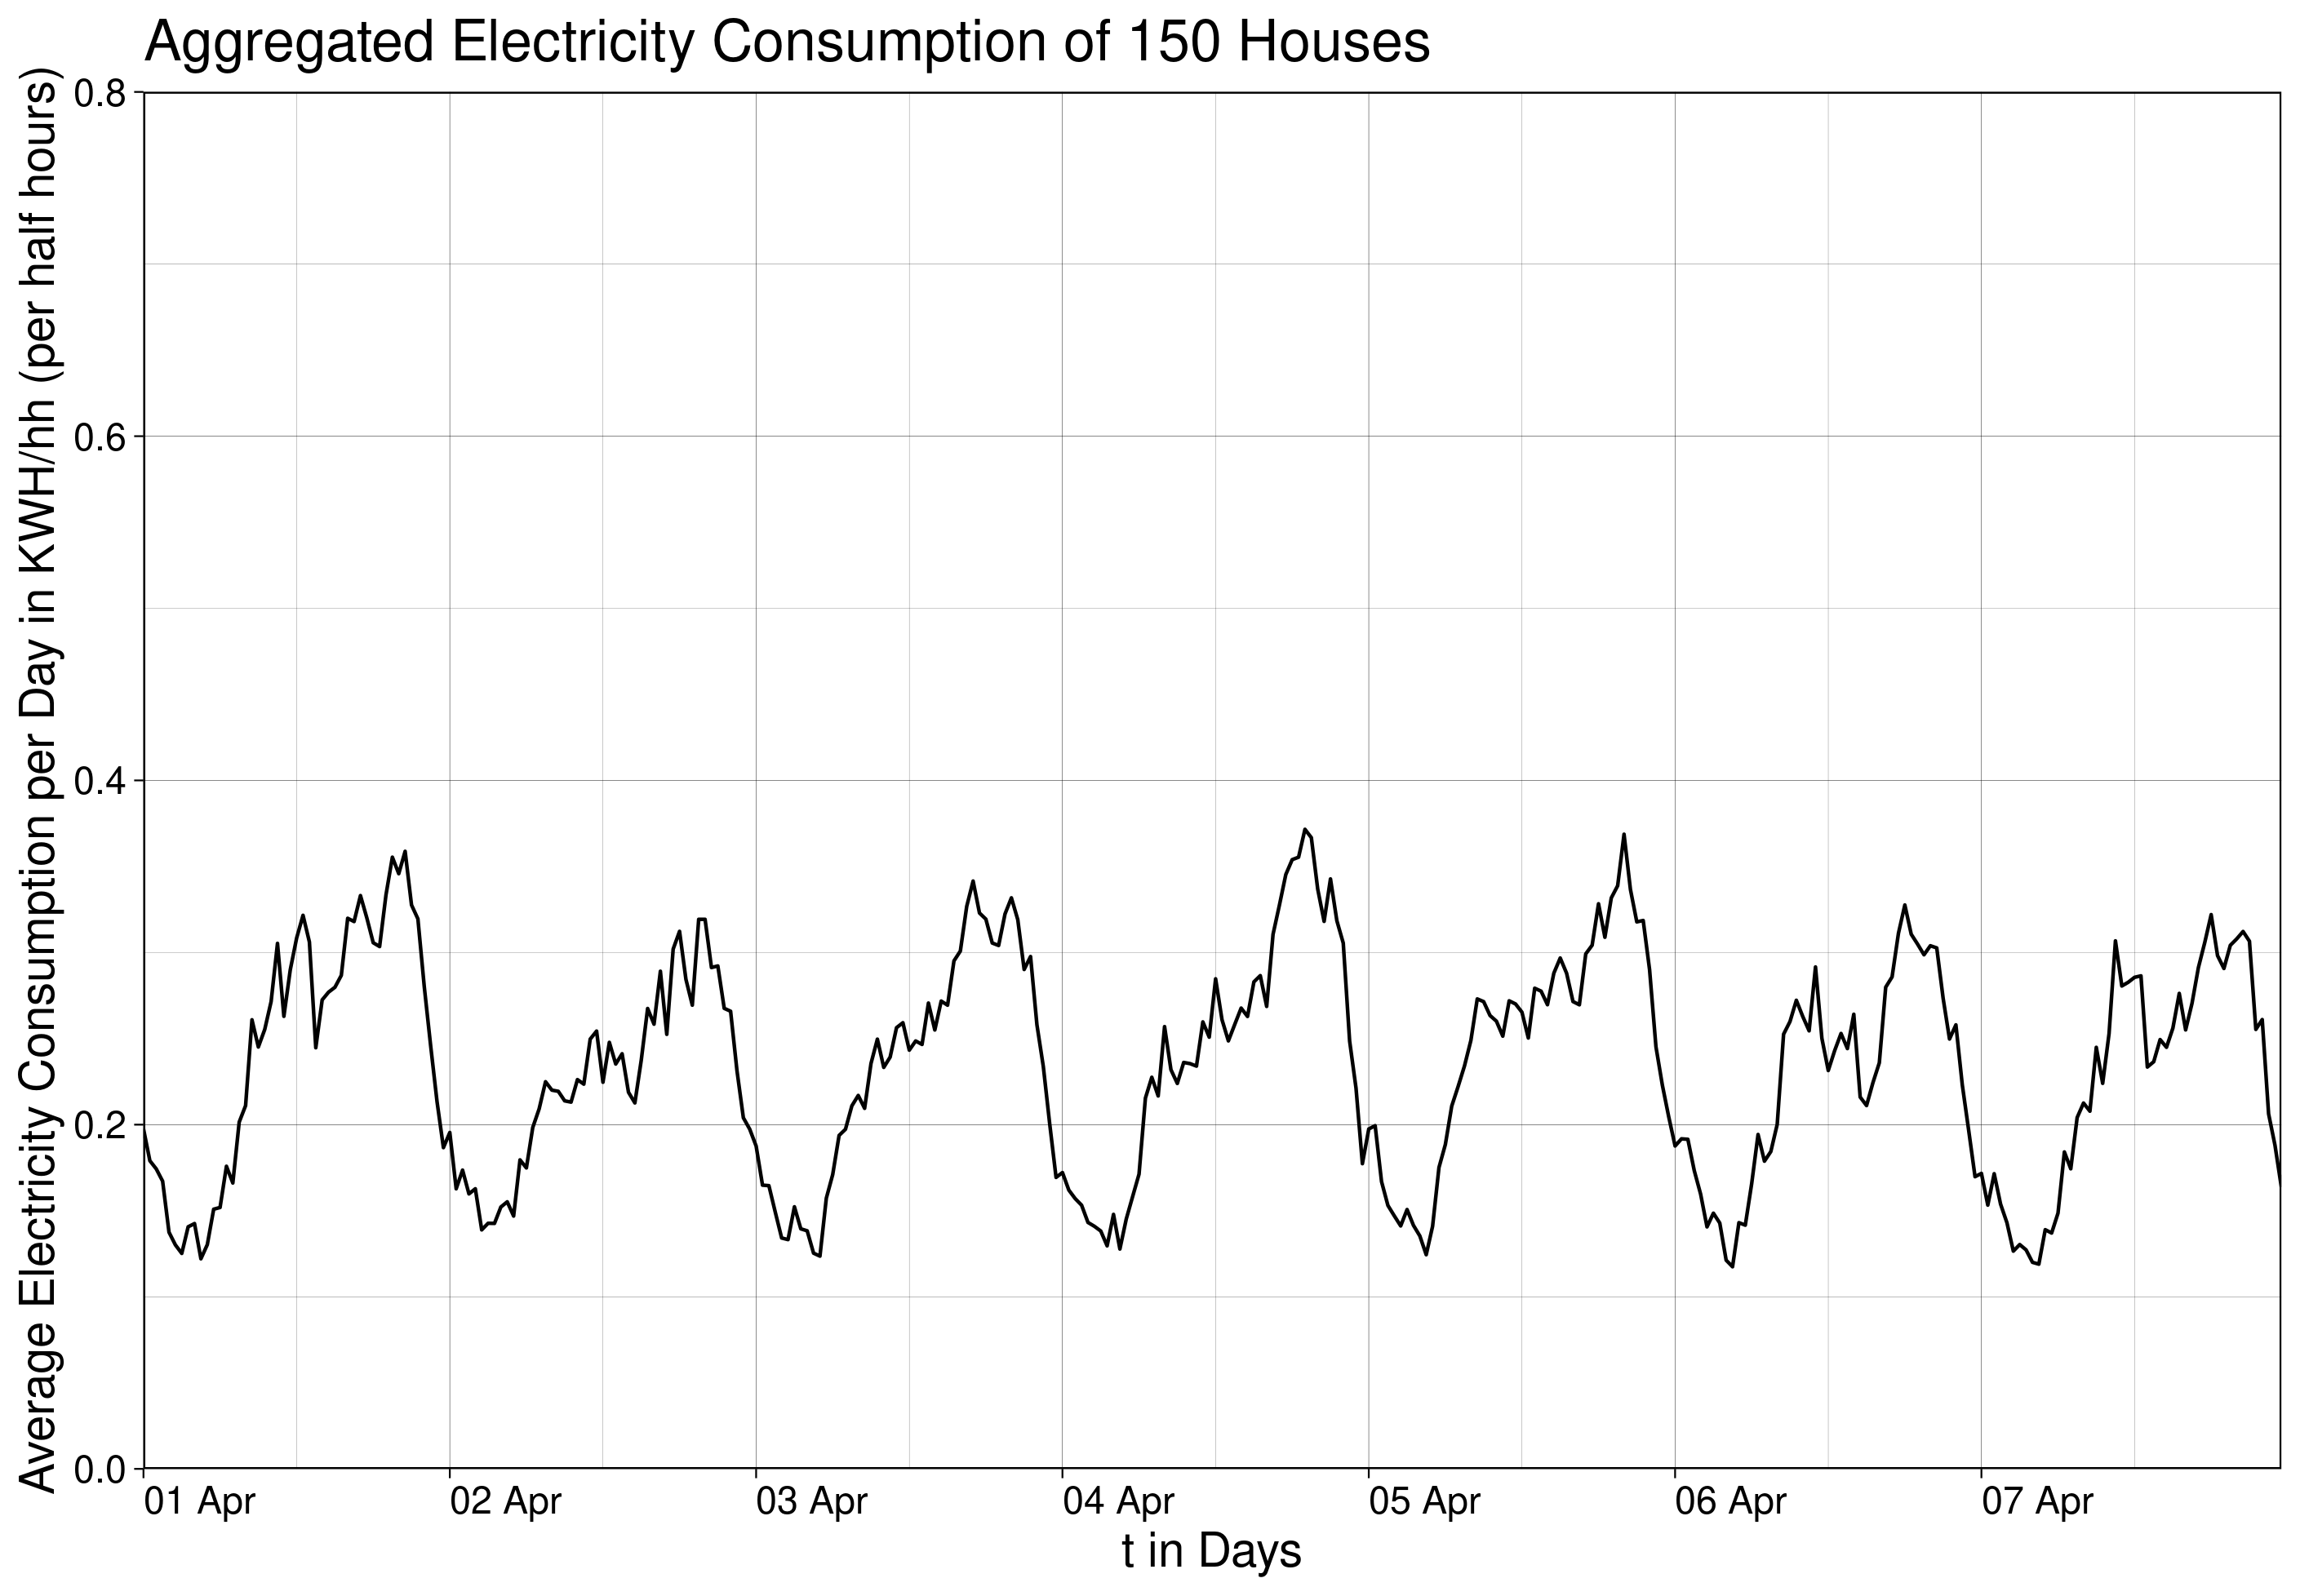
\includegraphics[width=0.85\textwidth]{images/Aggregated Electricity Consumption of 150 Houses5.png}
\caption[Aggregated Electricity Consumption of 150 Houses of the 2nd Experiment]{}
\label{img:150_houses_weekly}
\end{figure}
\clearpage
}

\afterpage{%
\begin{figure}[!p]
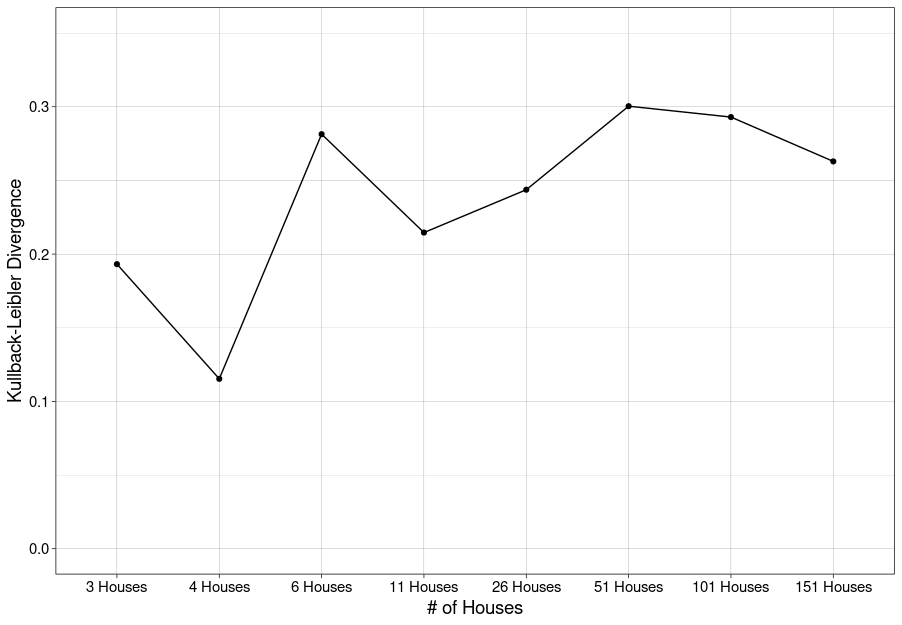
\includegraphics[width=0.85\textwidth]{images/KLD_Test2.png}
\caption[Kullback Leibler Divergence]{Kullback Leibler Divergence}
\label{img:KLD}
\end{figure}
\begin{figure}[!p]
\centering
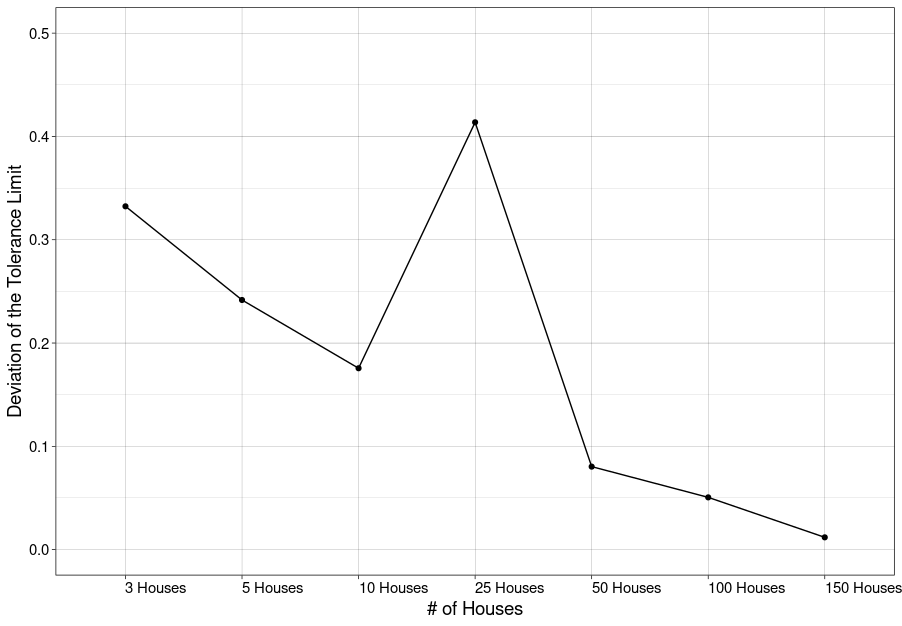
\includegraphics[width=0.85\textwidth]{images/Deviation1.png}
\caption[Deviation of the 2nd Experiment]{Deviation}
\label{img:Dev_2nd}
\end{figure}
\clearpage
}

